\section{Introduction}

\begin{figure*}[!t]
     \begin{minipage}{0.62\linewidth}
        \centerline{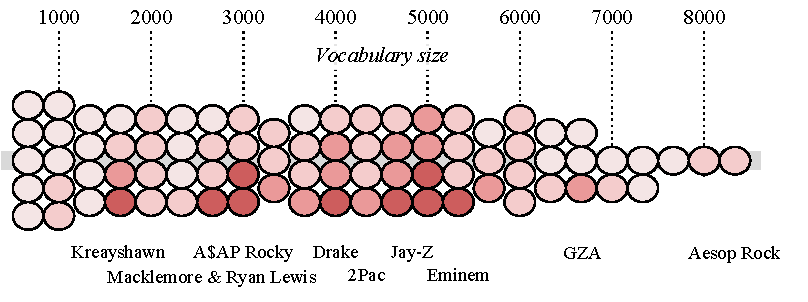
\includegraphics[width=0.99\linewidth]{figs-glossy/rappers_viz.pdf}}
        \vspace{-1ex}
        \caption{A visualization of rappers according to their vocabulary requires selecting the most popular rappers for each word bracket out of a much larger set of artists. The visualization should display more rappers as we zoom into word brackets for more detail. Note that even though the visualization organizes rappers in a word line (1-D), it uses the popularity dimension of the artist to both aid selection and to shade the surviving bubbles.}\label{fig:example:rappers}
    \end{minipage} \hfill
       \begin{minipage}{0.36\linewidth}
        \centerline{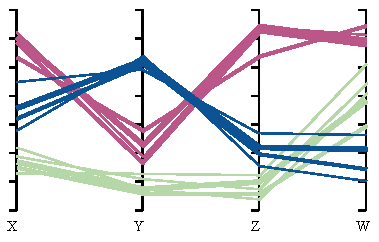
\includegraphics[width=0.99\linewidth]{figs-glossy/parallel_coordinates.pdf}}
        \vspace{-1ex}
        \caption{A visualization of k-means clusters with parallel coordinates requires us to limit to $n$ the number of lines that can cut through each dimension line segment for any vertical unit of space, at a scale-dependent resolution. Line widths are set by distances to cluster centers.} \label{fig:example:clusters}
    \end{minipage} \hfill
\end{figure*}

\begin{figure*}[!t]
     \begin{minipage}{0.62\linewidth}
        \centerline{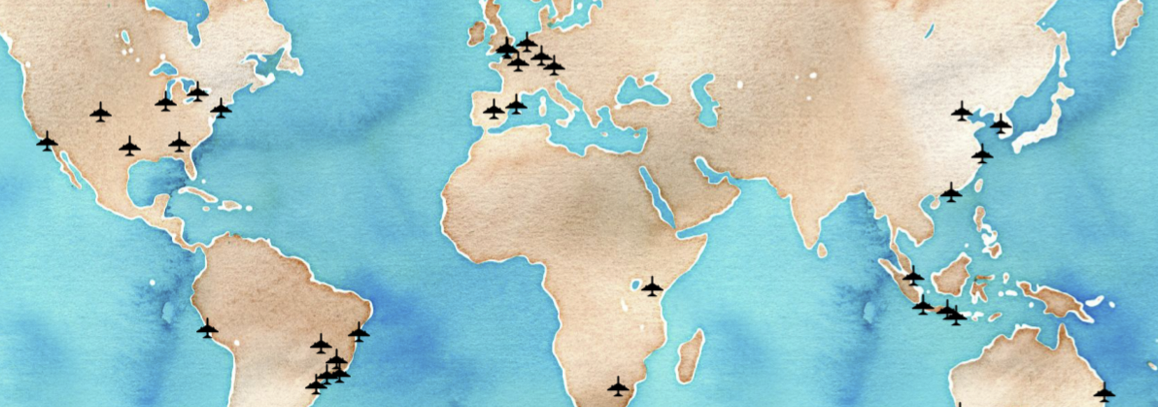
\includegraphics[width=0.99\linewidth]{figs-glossy/airports.png}}
        \vspace{-1ex}
        \caption{A visualization of airports in a geographical map requires the selection of the airports with the most traffic out of a larger set of airports. The visualization should display more airports as we zoom into geographical regions for more detail.}\label{fig:example:airports}
    \end{minipage} \hfill
       \begin{minipage}{0.36\linewidth}
        \centerline{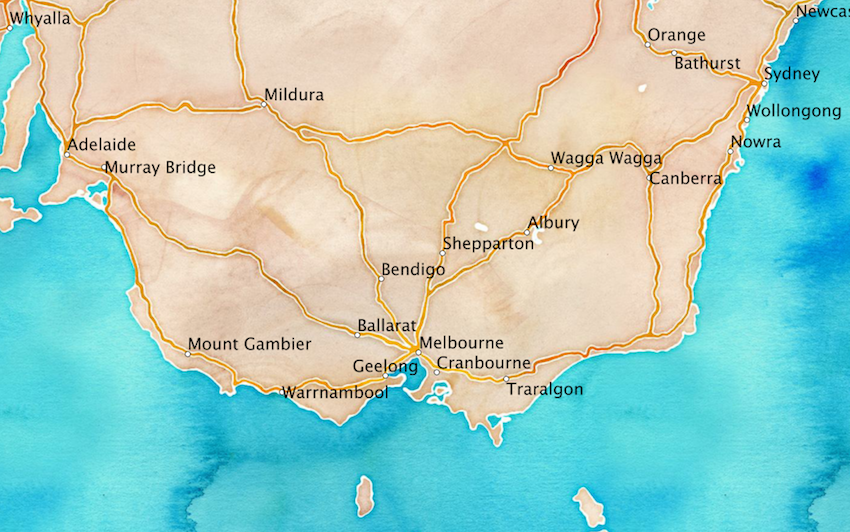
\includegraphics[width=0.96\linewidth]{figs-glossy/placenames_viz.png}}
        \vspace{-1ex}
        \caption{A visualization with placenames in a geographical map requires displaying or omitting labels according to scale.} \label{fig:example:placenames}
    \end{minipage} \hfill
\end{figure*}

We are faced with unprecedented data volumes in organizations across a wide variety of sectors~\cite{MCB+11:McKinsey}. In this context, data visualization of large and complex data is attracting renewed attention in data management and visual analytics~\cite{FeketeS12:DMVisChallenges,hanrahan:enthusiast,wu:case}. Computational journalism~\cite{CohenHT:2011:CompJournalism}, data science~\cite{KandelPHH12:InterviewStudy}, and citizen activism~\cite{ViegasM:2009:ManyEyes} are just a few examples of the new types of applications that require visualizations to help humans make sense of large datasets. To support these applications, it is crucial to abstract data in a way that reduces its volume, given that the amount of pixels in a display is often insufficient to convey detailed information about a large dataset.

Two of the most intuitive data reduction operations are to aggregate or select data. Data aggregation provides insights into the characteristics of datasets as a whole; however, this overview comes at the price of potentially losing valuable detail. Data selection, on the other hand, allows users to examine particular examples to get a more nuanced understanding of the data; however, this detail comes at the price of potentially being overwhelming. Recent studies indicate that data scientists find it difficult to express information needs for visualizations in existing query and programming languages, creating a substantial gap to be closed in current technology~\cite{KandelPHH12:InterviewStudy}.
 
Despite the wealth of existing work on data visualization, most systems have either focused on abstracting data by aggregation~\cite{blais:generating,LinsKS13:Nanocubes,StolteTH:2003:Multiscale,vartak:seedb}, or on devising techniques to squeeze a whole dataset into the available pixels~\cite{KeimK95:VisDB,KruskalW78:MDS}. The problem of creating visualizations that explicitly show representative items from a large underlying dataset has received far less attention. Nevertheless, the importance of this problem is significant. Figures~\ref{fig:example:rappers} to~\ref{fig:example:placenames} illustrate a few visualizations that crucially depend on data selection. These visualizations vary substantially in dimensionality, going from a single axis in the case of Figure~\ref{fig:example:rappers} to a parallel coordinates plot of multiple dimensions in Figure~\ref{fig:example:clusters} to two-dimensional geographical maps in Figures~\ref{fig:example:airports} and~\ref{fig:example:placenames}. Furthermore, these visualizations employ multiple scales to allow users to zoom into the data and see more records from the underlying dataset in an interactive fashion. Moreover, these visualizations are becoming ever more necessary for human understanding as we move towards an age of large datasets and data enthusiasts~\cite{hanrahan:enthusiast,markl:breaking}. Even though previous work has targeted particular examples of such visualizations, e.g., for spatiotemporal data~\cite{jugel:m4,KefaloukosSZ14:CVL,DasSarmaLGMH12:FusionTables}, a generic solution to multi-scale data selection has remained elusive. Such a solution should ideally be able to globally sample records, while respecting user-defined constraints and notions of record importance, and at the same time elegantly reuse database technology to operate on large datasets.   

In this paper, we introduce Glossy (GLObal Selection SYstem), a system that computes global selections over records stored in an RDBMS. In short, Glossy's novelty and utility rests on three pillars: (a) Glossy SQL, an extension of SQL that allows visualization developers to express global selection in a concise, yet familiar, query language, (b) an efficient translation of Glossy SQL into pure SQL, which allows Glossy to harness the power of mature query optimizers and indexed tables at runtime, (c) support for global selection over any type of tabular data, not just data within a certain domain (e.g., temporal or spatial data). With Glossy, multi-scale global selections of data for all the visualizations in Figures~\ref{fig:example:rappers}--\ref{fig:example:placenames} can be achieved concisely in a common declarative framework.  

\subsection{Our Contributions}

Having set the stage for our work above, we start by reviewing related approaches (Section~\ref{sec:related}). Then, the paper presents its main contributions:

\begin{enumerate}

\item Motivated by a wide range of use cases in data visualizations (Section~\ref{sec:use:cases}), we introduce Glossy SQL, an extension of SQL centered around the notion of global selections. We show how Glossy SQL can be used to declaratively express global selections for visualization use cases, as well as formally define single-scale and multi-scale global selections (Section~\ref{sec:global:selections}).  

\item Given a well-grounded understanding of the semantics of global selection, we proceed to present a translation of Glossy SQL into pure SQL. This translation allows for immediate use of Glossy SQL over existing RDBMS. In addition, it also allows Glossy to efficiently and scalably process global selection queries by reusing mature query processing technology (Section~\ref{sec:sql:translation}). 

\item In a set of experiments (Section~\ref{sec:experimental:evaluation}), we demonstrate that the Glossy SQL translation allows for: (a)~expressing a range of visualization use cases and efficiently executing them over an existing RDBMS, (b)~generating SQL code that is scalable on input sizes, and (c)~running a general global selection system that is generally superior in expressivity and performance to an existing data selection approach specialized to the domain of geographical maps. 

\end{enumerate} 

\section{Related Work}
\label{sec:related}

The problem of visualizing large datasets has been the subject of extensive research. While a comprehensive survey is beyond the scope of this paper, we categorize related approaches in the following and contrast them to Glossy. First, we discuss approaches to transforming data for and into visual representations. These data and visual abstraction approaches differ in whether they consider single-scale or multi-scale abstraction (Section~\ref{sec:related:abstraction}). Second, we turn our focus to recent visual analytics work, which has been covering the gamut from facilitating to speeding up data management tasks for visualizations (Section~\ref{sec:related:analytics}). Finally, we consider related work on data transformation for general multidimensional and specific spatiotemporal visualizations (Section~\ref{sec:related:multidimensional}). 

\subsection{Visual and Data Abstraction}
\label{sec:related:abstraction}

\minisec{Single-Scale Abstraction}
In information visualization, early approaches such as Fisheye~\cite{Sarkar:1994:Fisheye} or MagicLenses~\cite{BierSPBD93:MagicLenses} focused on specific information summarization schemes to help the user in navigating a large information space. Concurrent proposals such as XdmvTool~\cite{Ward:1994:XmdvTool} aimed at packaging common visualization components into libraries for developers. In the database community, extensible approaches have been pursued, e.g., Tioga-2~\cite{AikenCSW96:Tioga2}, RBE~\cite{KrishnamurthyZ95:RBE}, or DEVise~\cite{Livny:1997:DEVise}. In these extensible approaches, the developer would define both the data processing pipeline or query and a mapping to visual components. An important aspect was algebraic or declarative formalization of the allowable operations. In a similar vein, Polaris~\cite{StolteTH2008:Polaris} and its commercial successor Tableau~\cite{hanrahan:enthusiast} followed this type of approach, but went full circle in completing the mapping from visual components back to queries. In line with a recent vision for Data Visualization Management Systems~\cite{wu:case}, the latter approaches as well as Glossy build on declarative languages and database technology to scale processing of visualization functionality. However, as opposed to the approaches above, Glossy supports potentially complex, multi-scale visualizations.  

\minisec{Multi-Scale Abstraction}
DataSplash was designed to offer to developers the capability to design multiple canvases and to connect them with semantic zooming primitives, such as computing aggregates or changing visual representation~\cite{WoodruffOACELSS01:DataSplash}. While the approach is flexible, it requires substantial design effort to create complex visualizations. Approaches such as Nanocubes~\cite{LinsKS13:Nanocubes} or the data cube approach of Stolte et al.~\cite{StolteTH:2003:Multiscale} address this shortcoming by automatically adapting visual representation over an underlying data cube representation. These approaches are, however, focused on aggregation as their main data reduction operation. ScalaR applies a wider range of data reduction operations, such as filtering, aggregation, or sampling, to array data according to visualization scale~\cite{BattleSC13:DynamicReduction}. The approaches of Healy~\cite{Healey96:MultidimensionalViz} and Artero et al.~\cite{ArteroOL04:ClustersViz} abstract data by clustering algorithms. In contrast to Glossy, all of these approaches lack the capability to select representatives of a dataset in a manner that eliminates global visual conflicts and maximizes importance functions declaratively specified by the visualization developer.     

\subsection{Visual Analytics}
\label{sec:related:analytics}

\minisec{Facilitating Analytics}
Visualization in itself may not be an end-goal, but rather a tool for other activities in a data management pipeline. In particular, it has been recently proposed that data visualization help support interactive data wrangling~\cite{KandelPHH11:Wrangler}, data exploration and data management workflows~\cite{BavoilCSVCSF05:VisTrails,FeketeS12:DMVisChallenges}, as well as interactive data integration and cleaning~\cite{MortonBGM14:VisClean}. Our work dovetails with these approaches, by providing means for abstracting a fully or partially integrated dataset for multi-scale visualization.    

Recent systems have explored statistical techniques to both recommend visualizations as well as improve their computation time by approximation. VizDeck allows users to visually explore correlations among variables in a relational dataset by ranking and displaying multiple plots in a card game metaphor~\cite{KeyHPA12:VizDeck}. SeeDB helps the data analyst in the search for interesting trends in a subset of the data, where interestingness is measured by correlations that appear in the subset but not in the complete database~\cite{vartak:seedb}. The IFOCUS family of algorithms is closely related and complements this line of work by providing efficient sampling techniques that respect visual properties, such as ordering~\cite{blais:generating}. Sampling techniques have also been recently revisited to allow for efficient exploration of large datasets, with a focus on queries with simple aggregation operations~\cite{Agarwal:2014:blink,NirkhiwaleDJ13:sampling,SidirourgosKB11:SciBORQ}.  In contrast to this line of work, Glossy focuses on the problem of efficiently selecting data for a complex, potentially multi-scale, visualization rather than selecting and efficiently producing simple visualizations out of complex underlying correlations in a dataset. 

\minisec{Speeding Up Analytics}
A host of previous work, notably ParaView~\cite{HendersonAL04:ParaView}, VisReduce~\cite{ImVM13:VisReduce}, DICE~\cite{KamatJTN14:CubeExploration}, and imMens~\cite{LiuJH13:imMens}, focus on high performance, leveraging parallelism and incremental computation to speed up the computation of visualizations. However, unlike in Glossy, there is no notion of declarative data abstraction in these systems. Another system proposing a deep integration of visualization and data processing is dbTouch, in which touch actions are directly translated to database kernel operations~\cite{IdreosL13:dbTouch}. However, it is not clear whether the expressibility of such a system will be competitive with SQL.\newline

\subsection{Visualization of Multidimensional Data}
\label{sec:related:multidimensional}

\minisec{Multivariate Visualization}
Information visualization has pioneered a number of techniques for visualizing data in multiple dimensions, including scatterplot matrices, parallel coordinates, worlds-within-worlds, among others~\cite{CardMacS99:InfoVizBook,WongB94:InfoVizSurvey}. Many of these visualization techniques can benefit from Glossy's user-controlled data reduction before visualization. A subset of techniques, such as VisDB~\cite{KeimK95:VisDB} and multidimensional scaling~\cite{KruskalW78:MDS}, display data items by mapping them to a lower dimensional space based on their distances to a focal point or to each other. However, the premise behind these visualization techniques is squeezing as much of the dataset into the available pixels, leading to both loss of detail on data items as well as scalability limits with very large datasets. In contrast, Glossy gives users the capability to control data reduction declaratively, allowing for a user-defined compromise between scale, available pixels, and number of items selected for display.   

\minisec{Spatiotemporal Visualization}
The map drawing approach of Google Fusion Tables~\cite{DasSarmaLGMH12:FusionTables}, as well as some approaches from the cartography literature~\cite{NeunBW09:GeneralizationWeb,WareJT03:GeneralizationMeta}, model scale-sensitive data reduction as an optimization problem. However, unlike our approach, these methods work with algorithms that are specialized only to geographical data and that fail to integrate with DBMS technology. Jugel et al.~study how to perform data reduction for time series in the special case in which the visualization is a line chart, integrated with the underlying database via SQL queries in a system called M4~\cite{jugel:m4}. M4's approach can be seen as a particular case of global selection, in which up to four representative points are kept at each time segment according to visualization scale. Closer to our approach, the declarative cartography method of Kefaloukos et al.~proposes a multi-scale selection scheme specialized to geographical maps~\cite{KefaloukosSZ14:CVL}. We borrow from Kefaloukos et al.~the notion of visual conflicts and the algorithmic modeling of conflict resolution as a set multi-cover formulation. In contrast, Glossy extends not only to geographical data, but also to other types of visualizations in which representatives must be selected in a manner sensitive to scale. Moreover, we present a comprehensive SQL translation incorporating our generalized global selection semantics that allows for efficient reuse of existing DBMS~technology. Finally, within the domain of maps, we compare experimentally with the approach of Kefaloukos et al.~and show that the Glossy is generally superior not only in expressivity but also performance.    

%%%%%%%%%%%%%%%%%%%%%%%%%%%%%

\section{Use Cases}
\label{sec:use:cases}
While many datasets are small enough to be visualized directly, Glossy focuses on use cases that have a need for selecting multidimensional data points for legible, complex and explorable visualizations. We classify the examples on whether the visualization output is primarily organized around one dimension (Section~\ref{sec:examples:one:dimensional}), two dimensions (Section~\ref{sec:examples:two:dimensional}), or multiple dimensions (Section~\ref{sec:examples:n:dimensional}).  

\subsection{One-Dimensional Visualizations}
\label{sec:examples:one:dimensional}

Timelines are a prime example of a visualization technique organized around a single dimension. Glossy can easily handle the problem of data reduction for ``thin'' timelines, e.g., displaying the price of a stock or another single-variable function, by directly encoding the analysis of a recent study~\cite{jugel:m4}. However, a far more interesting use case for Glossy's global selection approach is visualizing ``broad'' timelines, i.e., timelines showing relevant events at each time frame. The example below illustrates such a use case.

\begin{example}[Historical events]
\label{ex:historical:events}
Consider a multi-scale visualization that shows a timeline of human civilization. Historical events are gathered into differently sized time buckets, e.g., centuries, decades and years, depending on the scale. For each bucket, we select the most important historical events.~To convey an impression of the activity level of each period, we select fewer events for buckets will low historical activity. \mathendbox
\end{example}

Non-temporal datasets can also be transformed for one-dimensional visualization. First, we must choose which axis in the dataset to explore. Then, we proceed in a  manner similar to the use case of a historical timeline. An example of non-temporal data selection is illustrated below, namely selecting musicians according to the size of their active vocabulary.

\begin{example}[Vocabulary Sizes]\label{ex:rappers}
Two aspects that distinguish musicians (e.g., rappers) are their popularity and the size of their vocabulary, as recorded in their lyrics. We can visualize these differences among artists by positioning rappers on a word-count line. The line is divided into buckets of word-count intervals and for each bucket we select the $k$ most popular rappers. If we zoom on the line, the interval sizes should become smaller, which consequently means that we get more buckets. This in turn means that we can select more rappers. To communicate that not all buckets have an equal amount of rappers who fall into their interval, we select fewer than $k$ for buckets that have low rapper counts. Finally, we would like to ensure that our favorite artist appears at all zoom levels regardless of the artist's popularity.~\footnote{Inspired by the visualization at~http://rappers.mdaniels.com.s3-website-us-east-1.amazonaws.com/. Figure~\ref{fig:example:rappers} is the result of reproducing their methodology over raw data sources, and employing Glossy SQL for data selection.} \mathendbox
\end{example}

The example of visualizing rappers described above is illustrated further in Figure~\ref{fig:example:rappers}.

\subsection{Two-Dimensional Visualizations}
\label{sec:examples:two:dimensional}

Digital maps are widely used to visualize geographical data that has been projected into two dimensions. From cartography, we know that spatial data must be abstracted according to scale in order to make a useful map~\cite{NeunBW09:GeneralizationWeb,WareJT03:GeneralizationMeta}. Advanced techniques are needed to abstract the topographical data, such as street networks and buildings, that compose the base maps exposed by a host of web services such as Google Maps.\footnote{http://maps.google.com} However, the far more interesting use cases of layering user data on top of these base maps are a perfect fit for the global selection approach of Glossy. Two examples of such spatial data are points of interest and place names. 

\begin{example}[Points of interest (POI)]
\label{ex:poi}
Points of interest (e.g., hotels or tourist attractions) are often shown on zoomable maps as an overlay on top of a background map. On a good POI map, items must not disappear when zooming in, a property referred to as zoom consistency~\cite{DasSarmaLGMH12:FusionTables}. In addition, modern maps are gridded into tiles at each scale, and web services often transfer tiles individually. It is thus natural to adopt tiles as a bucketing mechanism for information on a map. 
For each tile, we select at most $k$ POI prioritized by the number of positive reviews given to each POI (notice that this rank is scale-independent). Additionally, as each POI needs to be represented by a symbol, we should make sure not to select POI too close in space to each other, as measured by their scale-dependent distance in pixels on the map. \mathendbox
\end{example}

While points of interest should satisfy zoom consistency, this is not generally true of any overlay data. For placename labels, it would be odd to show the labels ``Italy'' and ``Europe'' on a map zoomed to a Roman neighborhood, even though Rome is situated in both Italy and Europe. Conversely, it would be odd to display the label ``Monti'', a Roman neighborhood, on a map of Europe, even though ``Monti'' is a part of Europe. An example of selecting this type of overlay data is given below.

\begin{example}[Placenames]
\label{ex:placenames}
To select placenames for a zoomable map, we assume that the territory associated with a label is represented by a crude polygon. Furthermore, we assume that we know the importance of each placename. For each scale and each map tile, we want to select at most $k$ labels prioritized by importance. Additionally, for a given scale, we only consider labels with a territory area that is roughly equal to the area of tiles at the given scale. While these labels may overlap, common functionality exists in most mapping software to rotate, displace and hide labels as needed. Consequently, we simply set $k$ high enough to account for possible label loss. \mathendbox
\end{example}

Displaying airports worldwide is a similar use case to displaying POI, illustrated further in Figure~\ref{fig:example:airports}. The example of placenames is illustrated in Figure~\ref{fig:example:placenames}. 

\subsection{N-Dimensional Visualizations}
\label{sec:examples:n:dimensional}

Visualizing the output of clustering algorithms such as k-Means is an interesting example of multidimensional visualization. One approach to visualize the result is to employ a multivariate visualization scheme such as parallel coordinates~\cite{CardMacS99:InfoVizBook,WongB94:InfoVizSurvey}. In the following, we show how to produce a multi-scale parallel coordinates visualization using global selection.

\begin{example}[Cluster representatives]\label{ex:clusters}
Assume we wish to visualize the results of running k-Means against a given multidimensional dataset. Each record contains an attribute with its corresponding cluster label. In a zoomable parallel coordinates plot, where records are represented by polylines, we may wish to limit to $n$ the number of polylines that can cut through each dimension line segment for any vertical unit of space, at a scale-dependent resolution. This procedure is similar to the one we employed for placenames and tiles in a map. In contrast, we may wish to rank records in a more interesting way: by taking their distance to the cluster centroid as a ranking function. \mathendbox
\end{example}

As we can see from these many examples, several patterns of data selection are reoccurring in a variety of visualization use cases of different dimensionality. Glossy's notion of global selection is designed to capture these patterns into an elegant syntax and well-defined semantics.  

\section{Global Selections}
\label{sec:global:selections}

In this section, we present the Glossy SQL extension. We begin by providing an overview of the features and syntax of Glossy SQL (Section~\ref{sec:syntax}), followed by Glossy SQL examples that solve the use cases of the previous section (Section~\ref{sec:use:cases:solved}). The semantics of Glossy SQL are then discussed (Section~\ref{sec:semantics}). 

\subsection{Overview and Syntax}
\label{sec:syntax}

The main idea of Glossy SQL is to give visualization developers control over how records are sampled from a large dataset in a manner sensitive to scale, but at the same time offer a general, concise, and declarative interface. To intuitively understand this new capability, consider that we could reduce the size of a large set of records by random sampling. However, as we have seen in Section~\ref{sec:use:cases}, random sampling would be insufficient for a number of visualizations. In many visualizations, we need to respect constraints, e.g., on the proximity between records or on the allowable record density on unit areas of the display. In addition, we also typically wish to represent in the display the most important records, ranked by a weighting function. 
The final result is still a sample of the input, albeit not a random~one. 

We may think of the process described above as a weighted, constrained sampling process. In relational terms, this process operates in a manner similar to a selection operator, filtering out records from the input that do not qualify well-defined conditions. However, unlike in a relational selection, the conditions on the records are not evaluated for each record independently, but for the set of records as a whole. Therefore, we call the operation specified by Glossy SQL a \emph{global selection}.

\begin{figure}[!t]
\begin{center}
\begin{lstlisting}
glossy_sql_stmt ::=
 SELECT
   {expression_list}
 FROM 
   {input_table} [AS {alias}] 
                 [ID BY {column_list}] 
   [ 
    {ITERATE OVER | RECURSE OVER}
      {scale_column_list} IN
      {RANGE FROM {bottom_value} TO {top_value} |
       SEQUENCE {tuple_list} |
       {subquery}} [AS {alias}]
   ]
 [WHERE {condition}]
 [WEIGH BY
   {float_expression}]
 [SUBJECT TO
   {constraint_list}] 	

constraint_list ::=
 {constraint} [AND {constraint_list}]
 
constraint ::=
 {pair_constraint} | {locus_constraint}
 
pair_constraint ::=
 FOREACH PAIR {left_var_name}, {right_var_name}   
  [WHERE {var_condition}]
  DROP [ONE | BOTH]

locus_constraint ::=
  FOREACH LOCUS
  MAP BY {expression}
  [FILTER BY {condition}]
  LIMIT {integer_expression} 
    [SCALE {LINEAR | LOG}] 
\end{lstlisting}
\vspace*{-2ex}
\caption{Syntax of Glossy SQL extension.}
\label{fig:glossy:sql:syntax}
\end{center}
\vspace*{-4ex}
\end{figure}

Figure~\ref{fig:glossy:sql:syntax} presents the syntax of Glossy SQL. The main features exposed through this syntax are discussed below. 

 \minisec{Representation of multiple scales} 
In contrast to standard SQL, Glossy SQL statements may specify an ordered table in an \textbf{\texttt{ITERATE OVER}} or a \textbf{\texttt{RECURSE OVER}} clause. This ordered table corresponds intuitively to information on the multiple scales in the visualization. For example, this table may correspond to a sequence of zoom levels, with attributes such as the pixel resolution. In an iterative query, the input given to each scale is the whole input table along with the information in the tuple for that scale in the ordered table. In a recursive query, by contrast, the global selection result at a given scale $s$ is the input to global selection at scale $s+1$.  

\minisec{Record weight and identity}
An important input to global selection is the weighting function used on the records of the input, given by the user in the \textbf{\texttt{WEIGH BY}} clause. For convenience, we also allow the user to specify a list of columns that acts as a key to the input records in the \textbf{\texttt{ID BY}} clause. While this information can be obtained from the catalog of many RDBMS, the option of specifying it allows for more flexibility in integrating data wrapped as relational and also for reduced effort in porting the translation of Glossy SQL to multiple database systems. 

\minisec{Control over visual conflicts}
Another important input to global selection is the specification of constraints that limit which records from the input can appear together in the final output. Informally, we say that a set of records are in a visual conflict if a constraint binds them together. There are two types of constraints in Glossy SQL: \emph{pair} and \emph{locus} constraints. A pair constraint binds together pairs of records in conflicts, where each conflict determines that either one or both of the records must be dropped from the output. A proximity constraint is an example of a pair constraint. In Figure~\ref{fig:constraints:schematic}(a), we visualize schematically the conflict structure created by a pair constraint.~Pair constraints allow for complex dependency structures among records as specified by a binary conflict relation.  

\begin{figure}[t]
\centering
\scalebox{0.48}{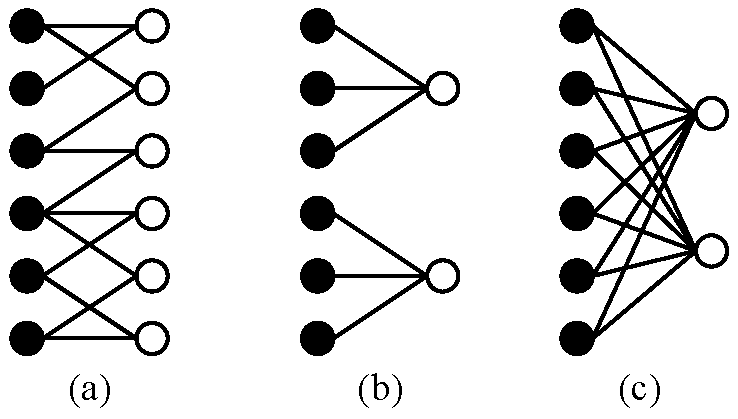
\includegraphics{figs-glossy/constraints.pdf}}
\vspace{-2ex}
\caption{Schematic representation of how records (solid circles) are organized into conflicts (empty circles) by different types of constraints: (a) A pair constraint, (b) A simple locus constraint, and (c) A complex locus constraint.} 
\label{fig:constraints:schematic}
\vspace{-2ex}
\end{figure}

A locus constraint binds together sets of records, where each set is informally the result of mapping the input records to a common identifier termed a locus. The set of loci can be thought of as a user-specified discretization of a space. For example, a density constraint is a locus constraint in which each locus corresponds to a unit area at a given scale. While a simple locus constraint uses a function that maps each record to exactly one locus, a complex locus constraint maps each record to a set of loci, i.e., the mapping function is a table function. The conflict structure of simple and complex locus constraints is illustrated in Figures~\ref{fig:constraints:schematic}(b) and~\ref{fig:constraints:schematic}(c).

By capturing in Glossy SQL multiple scales, record weighting, and constraint types that allow for natural specification of visual conflicts, we can concisely express the varied visualization use cases discussed in Section~\ref{sec:use:cases}.

\subsection{Examples: Solving the Use Cases}
\label{sec:use:cases:solved}

In this section, we show how to express the core use cases of Section~\ref{sec:use:cases} in Glossy SQL. While some use cases may seem different at first sight, a fair amount of commonality is exposed when they are expressed in Glossy SQL. For this reason, we omit detailed solutions when two use cases have substantially similar structure. 
We assume throughout this paper that input data is stored in a relational database system with appropriate indexing in place.  

\minisec{Rap artists selected by vocabulary size}
% About use case
We observe that Use Cases~\ref{ex:historical:events} and~\ref{ex:rappers} have essentially the same structure, and thus focus on presenting the Glossy SQL solution of Use Case~\ref{ex:rappers}.
To select rap artists for a zoomable line visualization based on vocabulary size, we employ a recursive Glossy SQL query, shown in Figure~\ref{fig:glossy:sql:rappers}. 

% Data details
The input table $rappers(\underline{id}, name, wordcount, pageviews)$ records information about each rap artist. While the meaning of the $id$ and $name$ columns is straightforward, the $wordcount$ column contains the number of distinct words used by an artist, obtained from an online lyrics database.\footnote{http://rap.genius.com} The $pageviews$ column contains the number of page views that the artist has received on the site; for this query, we use page views as a proxy for popularity.

% Query details
In the query, we use the \textbf{\texttt{RECURSE OVER}} construct to create a multi-scale global selection of rappers over five zoom levels. The construct implies that the output of a zoom level is used as input to the zoom level immediately lower. This ensures that data points will not disappear when zooming in, thus preserving zoom consistency. Each of the five scales are explicitly specified in the \textbf{\texttt{IN SEQUENCE}} clause. Each scale tuple has an integer $zoom$ column that can be used to select artists by scale later on, and an integer $bucketsize$ column that will control how rappers are grouped together into buckets.

While the outer \textbf{\texttt{WHERE}} clause specifies that we only select rappers with at least two songs, we further restrict the output by a locus constraint. In this constraint, we use the \textbf{\texttt{MAP BY}} clause to group rappers into buckets according to word count; rappers are mapped to buckets by arithmetic on the word count and bucketsize. For each bucket, we select at most 20 rappers and use \textbf{\texttt{SCALE LINEAR}} to maintain a linear density difference between dense and sparse buckets. As a final subtlety, we use a \textbf{\texttt{FILTER BY}} clause to ensure that our favorite band ``Digital Underground''  appears in the output, regardless of page views. Finally, we use the \textbf{\texttt{WEIGH BY}} clause to prioritize rappers based on their page views. 

% Query
\begin{figure}[!t]
\begin{center}
\begin{lstlisting}
SELECT id, name, wordcount, pageviews, zoom
FROM rappers ID id
   RECURSE OVER zoom, bucketsize 
   IN SEQUENCE 
   (5, 20), (4, 40), (3, 80), (2, 160), (1, 320)
WHERE songs > 1
WEIGH BY pageviews
SUBJECT TO
   FOREACH LOCUS
   MAP BY wordcount / bucketsize
   FILTER BY name <> 'Digital Underground'
   LIMIT 20 SCALE LINEAR
\end{lstlisting}
\vspace*{-2ex}
\caption{Selecting rappers on a line in Glossy SQL}
\label{fig:glossy:sql:rappers}
\end{center}
\vspace*{-5ex}
\end{figure}

\minisec{POI selected by star rating}
% About use case
To select points of interest (POI) for a zoomable map, our solution is another recursive Glossy SQL query, shown in Figure~\ref{fig:glossy:sql:poi}. However, in contrast to the previous example, a pair constraint is necessary to select POI with proper separation in 2-D. 
% Data details
In more detail, the input table $POI(\underline{id}, name, coord, stars)$ records the POI. The $coord$ column is a projected geographical coordinate, while the $stars$ column is a floating point value corresponding to the average star-rating given by reviewers.

% Query details
In the query, we use the \textbf{\texttt{RECURSE OVER}} syntax to create a multi-scale selection of POI over 19 zoom levels, which is a normal value for online maps. Again, the recursive selection guarantees that POI selected on lower zoom levels appear on all higher zoom levels. This time, we employ the \textbf{\texttt{IN RANGE}} clause to concisely specify the 19 integer values of the scales. Here, the $zoom$ column will be used both to enable selection of POI by scale later on, as well as to control the scale-dependent minimum proximity between POI that we will allow.

This time, we specify two constraints that restrict the selection, namely a locus constraint and a pair constraint. For the locus constraint, the \textbf{\texttt{MAP BY}} clause groups POI by map tile. This is achieved by the \texttt{TileCenter} function, which takes as input a point and a zoom level, and returns a label identifying the tile of the map in which the point is located at that zoom level. So in this example a locus corresponds to a tile. For each tile, we select at most 10 POI, and use \textbf{\texttt{SCALE LOG}} to maintain a logarithmic density difference between dense and sparse tiles. For the pair constraint, the \textbf{\texttt{WHERE}} clause specifies that two POI should not both be selected if they are in close proximity, measured in pixels in a scale-sensitive manner. Finally, we prioritize POI by their star-rating in the \textbf{\texttt{WEIGH BY}} clause. 

% Query
\begin{figure}[!t]
\begin{center}
\begin{lstlisting}
SELECT id, name, coord, stars, zoom
FROM poi ID id
   RECURSE OVER zoom 
   IN RANGE FROM 18 TO 0 
WEIGH BY stars
SUBJECT TO
   FOREACH LOCUS
   MAP BY TileCenter(coord, zoom)
   LIMIT 10 SCALE LOG
AND
   FOREACH PAIR x, y
   WHERE 
       DistancePixels(x.coord, y.coord, x.zoom) < 10
   DROP ONE
\end{lstlisting}
\vspace*{-2ex}
\caption{Selecting POI on a map in Glossy SQL}
\label{fig:glossy:sql:poi}
\end{center}
\vspace*{-5ex}
\end{figure}

\minisec{Placenames selected by relevance}
% About use case
To select placename labels for a zoomable map, we use an iterative Glossy SQL query, shown in Figure~\ref{fig:glossy:sql:placenames}. Since the query is iterative, the whole input is processed by the global selection at each zoom level, which allows labels to appear and disappear when zooming in. Additionally, we use a scale-dependent \textbf{\texttt{WHERE}} clause to remove labels that are irrelevant at a given scale.

% Data details
The input table $placenames(\underline{id}, label, polygon, importance)$ records the named places and their labels. The $label$ column records simply a text string, e.g., ``New York'' or ``Victoria''. The $polygon$ column is a geographical polygon that delineates the named place (e.g., continent, country or city). The $importance$ column records a user-defined weight for the label, e.g., a label for ``New York, NY'' is arguably more important than a label for ``White Plains, NY'', even though one is right next to the other.

% Query details
As stated above, we use the \textbf{\texttt{ITERATE OVER}} syntax in the query to allow placenames to be replaced by others when zooming in on the map. We combine this clause with the same \textbf{\texttt{IN RANGE}} clause that we use for the POI map. The query specifies a single locus constraint to ensure that we select at most $10$ labels per tile. Note that because the geometry of a named place is a polygon, this geometry may intersect many map tiles. So we use the \texttt{TileCenters} table function instead of the \texttt{TileCenter} function above so that we can map a given placename record to all the tiles that it intersects, again using tile labels as loci.  
Finallly, the \textbf{\texttt{WEIGH BY}} clause is used to rank labels according to their importance. 

% Query
\begin{figure}[!t]
\begin{center}
\begin{lstlisting}
SELECT id, label, polygon, importance, zoom
FROM placenames ID id
   ITERATE OVER zoom 
   IN RANGE FROM 18 TO 0
WHERE Area(polygon) / TileSize(zoom) 
      BETWEEN 0.1 AND 4
WEIGH BY importance
SUBJECT TO
   FOREACH LOCUS
   MAP BY TileCenters(polygon, zoom)
   LIMIT 10
\end{lstlisting}
\vspace*{-2ex}
\caption{Selecting placenames on a map in Glossy SQL}
\label{fig:glossy:sql:placenames}
\end{center}
\vspace*{-4ex}
\end{figure}

\begin{figure}[t]
\centering
\scalebox{0.25}{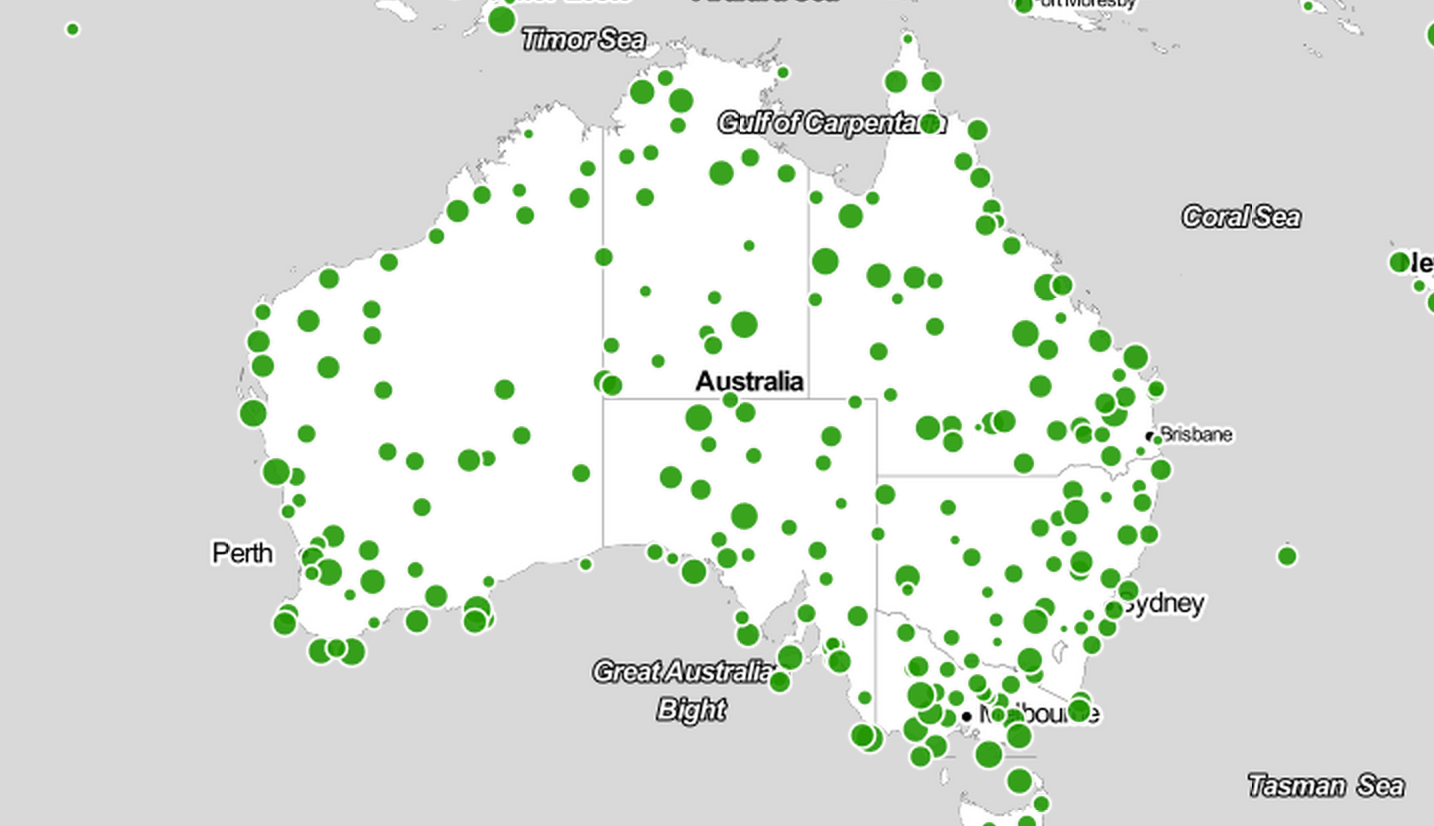
\includegraphics{figs-glossy/tourism_viz.png}}
\vspace{-1ex}
\caption{Combined visualization of POI and placenames.} 
\label{fig:tourism:viz}
\vspace{-2ex}
\end{figure}

\minisec{Additional Examples}
While the examples above illustrate the main features of Glossy SQL, they do not exhaust the whole gamut of possibilities. For example, consider that in most of the previous examples, one query was used to prepare all the necessary data for a given visualization. However, this does not need to be the case. Figure~\ref{fig:tourism:viz} shows a visualization that combines both POI and placenames in a single map. The visualization is constructed by taking the queries from the previous two examples and using the results of each as a layer in the visualization. 

Also, as discussed in Section~\ref{sec:use:cases}, not all visualizations are primarily structured around one or two dimensions. The use case of Example~\ref{ex:clusters} describes a multidimensional visualization using parallel coordinates. The data selection for that visualization can be accomplished in Glossy SQL by employing one locus constraint for each axis, limiting the number of lines crossing each unit area in a manner similar to what is done in Figure~\ref{fig:glossy:sql:rappers}. Weighing by distance to a cluster centroid can be expressed simply as a scalar subquery joining against a $centroids$ table. 

For brevity, we focus on the examples of Figures~\ref{fig:glossy:sql:rappers} to~\ref{fig:glossy:sql:placenames} when further evaluating our approach; however, they are representative of a much broader class of visualizations expressible in Glossy SQL.    

\subsection{Semantics}
\label{sec:semantics}
% Discussion:
% Semantics are to satisfy constraints, which includes the empty solution.
% Specifically, there may be several valid solutions to a Glossy query
% To make it more meaningful, we incorporate minimising loss of weight

% We are presenting Glossy as an extension of SQL. Important that 
% the semantics of e.g. SELECT, WHERE, FROM, etc remain the same as in SQL.

Armed with the intuitive understanding developed above, we formalize the semantics of Glossy SQL in this section. The semantics for a single scale is specified in terms of a global selection operator $\Sigma$ in Section~\ref{sec:semantics:global:selection}. Based on this specification, Section~\ref{sec:semantics:multiscale} defines the semantics of multi-scale global selection.

\subsubsection{Global Selection Operator}
\label{sec:semantics:global:selection}

We first focus on the semantics of single-scale Glossy SQL queries, i.e., queries that include neither an \textbf{\texttt{ITERATE OVER}} nor a \textbf{\texttt{RECURSE OVER}} clause. The main features of single-scale queries are then the specification of a set of constraints as well as of a weighting expression over the records of the input table. These specifications are holistically combined into a global selection of the records of the input table.

We abstract the weighting expression by a function $w: \mathbb{T} \; \rightarrow \; \mathbb{R}_{0}^+$, where $w$ maps a tuple from the domain of all possible tuples $\mathbb{T}$ to a nonnegative real value.\footnote{The domain of all possible tuples in a relation $\mathbb{T}$ can be defined in the usual way by the cartesian product of the domains of the corresponding relation schema's attributes~\cite{RG02:CowBook}.} To model how constraints influence global selection, we must introduce the notion of a conflict. 

\begin{definition}[Conflict]
A conflict is a 2-tuple $c = (k, R)$, where $k \; \in \; \mathbb{N}$ is the maximum number of records that are allowed to survive after the global selection from the conflict $c$, and $R$ is a set of records from the input table with $|R| > k$. \mathendbox
\end{definition}
 
A conflict thus captures a set of records out of which only $k$ may be presented in the visualization. As we have seen in Section~\ref{sec:use:cases:solved}, these conflicts are typically associated with visual restrictions such as information density. 
 
A constraint $K$, when applied to an input relation $I$, specifies a set of conflicts $C$. The precise set of conflicts $C$ is defined according to the whether the constraint is a pair or a locus constraint. 

\begin{definition}[Conflict set for pair constraint]
A pair constraint $K$ defines a set of conflicts $C = \{ (k_1, R_1), (k_2, R_2), \ldots, (k_n, R_n) \}$ over an input relation $I$, where:
\begin{enumerate}[label=(\alph*)]
\item all $k_i = 1$ if the constraint's \textbf{\texttt{DROP}} clause specifies \textbf{\texttt{ONE}}, or all $k_i = 0$ if the \textbf{\texttt{DROP}} clause specifies \textbf{\texttt{BOTH}};
\item the $R_i$ contain exactly a pair of records each, corresponding to the records from the input relation paired by the join $I \bowtie_{Cnd} I$, where $Cnd$ is the condition specified in the constraint's \textbf{\texttt{WHERE}} clause. \mathendbox
\end{enumerate}   
\label{def:conflict:set:pair}
\end{definition} 

\begin{definition}[Conflict set for locus constraint]
A locus constraint $K$ defines a set of conflicts $C = \{ (k_1, R_1), (k_2, R_2), \ldots, (k_n, R_n) \}$ over an input relation $I$, where:
\begin{enumerate}[label=(\alph*)]
\item each $(k_i, R_i)$ corresponds to the conflict in exactly one locus $l_i$;
\item the possible loci $l_i$ are given by a set of labels $\mathbb{L}$, and the mapping of records to loci is given by a non-injective, non-surjective mapping function $f: \mathbb{T} \rightarrow \mathcal P (\mathbb{L})$ specified in the constraint's \textbf{\texttt{MAP}} clause, where $\mathcal P (\mathbb{L})$ is the power set of $\mathbb{L}$;
\item each record must be mapped to at least one locus;
\item when a record is mapped to multiple loci, it appears in the $R_i$ of the conflicts corresponding to each of these loci, when no \textbf{\texttt{FILTER BY}} clause is given;
\item when a \textbf{\texttt{FILTER BY}} clause is given, it is further ensured that none of the records in $R_i$ violate the condition $Cnd$ specified in the constraint's \textbf{\texttt{FILTER BY}} clause;
\item the values of $k_i$ are given by evaluation of the integer expression in the constraint's \textbf{\texttt{LIMIT}} clause, when no \textbf{\texttt{SCALE}} clause is given;
\item when a \textbf{\texttt{SCALE}} clause is given, the values of $k_i$ are scaled either linearly or a logarithmically as a fraction of the maximum value of all $k_i$ as defined above without scaling. 
\mathendbox 
\end{enumerate}
\label{def:conflict:set:locus}
\end{definition} 
 
Assume a Glossy SQL query is composed of constraints $\langle K_1, K_2, \ldots, K_m\rangle$, with associated sets of conflicts $\langle C_1, C_2, \ldots, C_m\rangle$ over the input. We define the conflict set of the query to be $\mathbb{C} = C_1 \;\cup\; C_2 \;\cup\; \ldots \; C_m$. Given a conflict set $\mathbb{C}$ over an input relation $I$, and a weighting function $w$, we can define the global selection operator as:
 
 \begin{definition}[Global Selection Operator]
The~global selection operator $\Sigma_{\mathbb{C}}^{w}: \mathbb{I} \rightarrow \mathbb{I}$, where $\mathbb{I}$ is the power set of $\mathbb{T}$, maps an input relation instance $I \; \in \; \mathbb{I}$ to an output relation instance $O \subseteq I$ s.t.:
\begin{enumerate}[label=(\alph*)]
\item $O$~contains at most $k_{i}$ surviving records for each of the conflicts $c_{i} = (k_{i},R_{i}) \; \in \; \mathbb{C}$;
\item the sum of the record weights in $O$ is maximal wrt.~all such qualifying relation instances.  \mathendbox 
\end{enumerate}
 \end{definition} 

Our notions of a visual conflicts as well as of finding a maximal-weight solution that resolves all conflicts are similar to the ones introduced by Kefaloukos et al.~\cite{KefaloukosSZ14:CVL}. It is easy to see that their conclusion that finding such a solution is equivalent to the set multi-cover problem also applies to the global selection operator. Since this problem is NP-hard, we relax the semantics of global selection to allow for the use of heuristics or approximate algorithms to compute global selection solutions. In contrast to~\cite{KefaloukosSZ14:CVL}, however, our definitions above constitute a general framework that transcends the visualization of geographical maps.     

To complete the description of the semantics of single-scale Glossy SQL queries, we observe that the \textbf{\texttt{SELECT}} clause is equivalent to a projection over the input table. So a single-scale Glossy SQL query over input relation $I$, with weighting function $w$, constraints $\langle K_1, K_2, \ldots, K_m\rangle$ yielding an associated set of conflicts $\mathbb{C}$, a \textbf{\texttt{WHERE}} clause with condition $Cnd$, and projecting attributes $\langle a_1, a_2, \ldots, a_l \rangle$ corresponds to the expression $\pi_{\langle a_1, a_2, \ldots, a_l \rangle} (\Sigma_{\mathbb{C}}^{w}(\sigma_{Cnd}(I)))$ in the extended relational algebra with the global selection operator. 
 
\subsubsection{Multi-Scale Global Selection}
\label{sec:semantics:multiscale}

We now turn to the semantics of multi-scale Glossy SQL queries. These queries include either an \textbf{\texttt{ITERATE OVER}} or a \textbf{\texttt{RECURSE OVER}} clause, which specify a sequence $S$ of tuples with the same schema s.t.~each tuple encodes information about a given scale. Multi-scale Glossy SQL queries apply a global selection at each scale, but construct the input for each scale differently according to whether they are iterative or recursive.

\begin{algorithm}
\caption{Conceptual Evaluation of Multi-Scale Glossy SQL.}
\begin{algorithmic}
\STATE $R \leftarrow I$
\STATE $O \leftarrow \emptyset$
\FOR{Tuple $t$ in $S$}  
\STATE $L_I \leftarrow \sigma_{Cnd}(t \times R)$
\STATE Derive set of conflicts $\mathbb{C}$ from $\langle K_1, K_2, \ldots, K_m\rangle$ and $L_I$
\STATE $L_O \leftarrow \Sigma_{\mathbb{C}}^{w}(L_I)$ 
\IF{\textbf{\texttt{RECURSE OVER}} $S$}
\STATE $R \leftarrow \pi_{\langle i_1, i_2, \ldots, i_p \rangle} L_O$ 
\ENDIF
\STATE $O \leftarrow O \; \cup \; L_O$
\ENDFOR
\RETURN $\pi_{\langle a_1, a_2, \ldots, a_l \rangle} (O)$
\end{algorithmic}
\label{alg:conceptual:multiscale}
\end{algorithm}

The semantics of multi-scale Glossy SQL queries can be specified by a conceptual evaluation program, as shown in Algorithm~\ref{alg:conceptual:multiscale}. Similarly to the single-scale case, we assume a query over input relation $I$ with attributes $\langle i_1, i_2, \ldots, i_p \rangle$, with weighting function $w$, constraints $\langle K_1, K_2, \ldots, K_m\rangle$, a \textbf{\texttt{WHERE}} clause with condition $Cnd$, and projecting attributes $\langle a_1, a_2, \ldots, a_l \rangle$.   


The algorithm iterates over the sequence $S$ one tuple at a time. Each tuple is cross-joined with the the current input tuples in $R$. In the case of an iterative multi-scale Glossy SQL query, these input tuples always correspond to the entire input relation $I$; in the case of a recursive multi-scale Glossy SQL query, however, the input tuples in $R$ correspond to the surviving tuples from the global selection of the previous scale. The algorithm derives the conflict set $\mathbb{C}$ from the constraints in the query in a way that is sensitive to the current input and scale. This process consists of producing conflict sets consistent with Definitions~\ref{def:conflict:set:pair} and~\ref{def:conflict:set:locus} from the previous subsection, but considering $L_I$ as the input relation. The output for the current scale $L_O$ is the result of the global selection over $L_I$ with conflict set $\mathbb{C}$ and weighting function $w$. This partial output is collected into a global output relation, which is projected according to the query before the final result is produced.  

\section{Pure SQL Translation}
\label{sec:sql:translation}

In this section, we present the translation of the Glossy SQL syntax introduced in Section~\ref{sec:syntax} to SQL. Without loss of generality, we conform to the SQL dialect and function library offered by PostgreSQL\footnote{http://www.postgresql.org/}, as used in the implementation of Glossy. Extension to other relational DBMS is conceptually straightforward.  

We start by discussing the translation of single-scale global selections in Section~\ref{sec:translation:global:selection}. Based on this translation, we present how to express in SQL multi-scale global selections in Section~\ref{sec:translation:multiscale}.  

\subsection{Global Selection Operator}
\label{sec:translation:global:selection}

We first discuss how to compute in SQL the elements that should be kept at a single scale. As discussed in Section~\ref{sec:semantics}, the global selection operator $\Sigma_{\mathbb{C}}^{w}$ specifies this single-scale computation, encoding the resolution of a set of visual conflicts $\mathbb{C}$ weighed by a weighting function $w$. The weighting function $w$ is directly specified in the Glossy SQL extended syntax through the \textbf{\texttt{WEIGH BY}} clause. The set of conflicts $\mathbb{C}$, on the other hand, must be derived from the constraints specified in the \textbf{\texttt{SUBJECT BY}} clause. Once $\mathbb{C}$ is derived, it is necessary to resolve all conflicts automatically by picking records to be deleted through an appropriate algorithm.  

Section~\ref{sec:calc:conflicts} examines how to compute $\mathbb{C}$ from the constraints, while Section~\ref{sec:resolve:conflicts} reviews algorithmic approaches to globally resolving conflicts. 

\subsubsection{Calculating the Set of Conflicts $\mathbb{C}$}
\label{sec:calc:conflicts}

We examine below how to translate both pair as well as locus constraints to SQL statements that derive conflict sets. To do so, some notation is required. The translation of Glossy SQL fragments is denoted by $\denote{$\cdot$}_E$, where $E$ is an environment. An environment is a set containing mappings of variable names given in a constraint to appropriate table aliases in the generated SQL. For simplicity, we omit specification of the environment in contexts where variable mappings are not required.  

The input to conflict calculation is the input table, potentially augmented with fields from the scale column list (see syntax in Figure~\ref{fig:glossy:sql:syntax}). Below, we assume that the scale to which the global selection is currently being applied be determined by an \texttt{iteration} column added to the augmented input table \texttt{current\_input}. Details on the augmentation process are given in Section~\ref{sec:translation:multiscale}. 

\minisec{Pair Constraints}
We start by examining pair constraints. Every conflict specified by a pair constraint involves two records from the input table, identified by the key given in the schema or explicitly in the \textbf{\texttt{ID BY}} clause (in case a key is not given, our translator generates a surrogate automatically). We assume for simplicity that the key is given by a column \texttt{K} of \texttt{current\_input}. Likewise, we assume that the weight is calculated into a column \texttt{weight}.  

Intuitively, generating pairs is a self-join operation on the \texttt{current\_input} table, and each pair represents a conflict that can be resolved by letting either one record survive or none.~This intuition is captured by the translation below: \\

\denote{\lstinline!FOREACH PAIR!$\;x,\;y\;$\lstinline!WHERE!$\;C\;$\lstinline!DROP ONE!} =
\begin{lstlisting}[mathescape,escapechar=!]
   SELECT
     -- conflict identifier is {cid, iteration}
     -- climit states max survivors
     l.K || '_' || r.K AS cid,
     l.iteration AS iteration,
     1 AS climit,
     -- record information
     Unnest(array[l.K, r.K]) AS rid,
     Unnest(array[l.weight, r.weight]) AS weight
   FROM current_input l JOIN current_input r
   ON   l.K < r.K AND
        l.iteration = r.iteration AND
        !\denote{$C$}$_{\{x \rightarrow l,\;y \rightarrow r \}}$!
\end{lstlisting}

The SQL statement returns sets of conflicts containing two records each, generated as expected by a self-join, and stating in the \texttt{climit} attribute that a single surviving record will resolve the conflict. The \texttt{Unnest} function creates one output record for each element in the given array. The translation of the \textbf{\texttt{WHERE}} clause must include the appropriate translation of the condition supplied by the user, taking into account the variable names $x$ and $y$. Note that omitting the \textbf{\texttt{WHERE}} clause above is equivalent to specifying the condition \textbf{\texttt{true}}, while specifying the clause \textbf{\texttt{DROP BOTH}} would yield instead a value of zero for the \texttt{climit} column returned by the SQL statement.
 
\minisec{Locus Constraints}
We now consider locus constraints. In a locus constraint, records are filtered by a constraint-specific \textbf{\texttt{FILTER BY}} clause, if one is provided. Then, a non-injective non-surjective function $f$ of records to sets of loci is applied, i.e., the application of $f$ results in each record being mapped to a set of loci, and thus each locus can potentially contain one or more records. Since conflicts are defined as loci with excessive numbers of records, resolving conflicts consists of reducing the number of records in each locus to at most the number $k$ given in the \textbf{\texttt{LIMIT}} clause. \\

\denote{\lstinline!FOREACH LOCUS MAP BY!$\;f(x)\;$\lstinline!  FILTER BY!$\;C\;$\lstinline!LIMIT !$\;k$} =
\begin{lstlisting}[mathescape,escapechar=!]
   SELECT
    !\denote{$f(x)$}$_{\{x \rightarrow c\}}$! AS cid,
    iteration AS iteration,
    !\denote{$k$}! AS climit,
    Unnest(array_agg(K)) AS rid,
    Unnest(array_agg(weight)) AS weight
   FROM current_input c
   WHERE !\denote{$C$}$_{\{x \rightarrow c\}}$!
   GROUP BY !\denote{$f(x)$}$_{\{x \rightarrow c\}}$!, iteration
   HAVING count(*) > !\denote{$k$}!
\end{lstlisting} 
 
The SQL statement applies the function $f$ to obtain one or many loci, depending on whether $f$ is defined as a simple function or as a table function. Each of the locus labels returned by $f$ serves both as a conflict identifier and as a grouping value. Similarly to the translation of a pair constraint, the SQL statement employs \texttt{Unnest} to expand the multiple input records mapped to the same conflict identifier into a corresponding number of output records, and the \texttt{iteration} column to separate conflicts in different scales. In addition, in the translations of the application of $f$ and of the condition $C$, we assume the variable $x$ is the alias specified for the input table in the query, which needs to be mapped accordingly. In the case of a multi-scale query with a separate alias for the sequence of scales, the environment mapping simply needs to be extended by this additional alias. 

\minisec{\texttt{SCALE} Clause}
Recall from Figure~\ref{fig:glossy:sql:syntax} that an optional \textbf{\texttt{SCALE}} clause may be specified for a locus constraint. Since the number $k$ given in the \textbf{\texttt{LIMIT}} clause is a hard bound, it is often the case that some loci will require that far more records be eliminated to resolve conflicts than others. For example, with a limit of 16 records per locus, loci with 20 records and 40 records will lead to deletion of 4 and 24 records respectively. This asymmetry may destroy distributional properties that some visualizations require to be maintained. In order to deal with this issue, the \textbf{\texttt{SCALE}} clause specifies that the limit bound should be scaled dynamically according to the maximum number of records in any given locus. The adjustment may follow either a linear or a logarithmic function.  

Specification of a \textbf{\texttt{SCALE}} clause affects the SQL translation above by replacing \denote{$k$} in the \texttt{climit} attribute with an appropriate expression involving a scalar subquery. In the case of \textbf{\texttt{LINEAR}} scaling, the resulting expression is:

\begin{lstlisting}[mathescape,escapechar=!]
  ceil(!\denote{$k$}!*(count(*)::float / 
             (SELECT max(cnt)
              FROM 
               (SELECT iteration, count(*) AS cnt 
                FROM current_input c1
                WHERE !\denote{$C$}$_{\{x \rightarrow c1\}}$!
                GROUP BY !\denote{$f(x)$}$_{\{x \rightarrow c1\}}$!,iteration) m              
              WHERE m.iteration = c.iteration)           
\end{lstlisting} 

%\kostas{Rewrote above SQL to shorter and equivalent query (I think). Need to verify.}

The scalar query scales the number of allowed survivors in each locus by the fraction of the number of records in the locus over the maximum number of records in any locus, within the same iteration. As can be seen from the query above, a simple and intuitive feature for a declarative language for visualizations can lead to a substantially complex underlying translation. The translation for logarithmic scaling is similar, but takes $\max(1,\log(y))$ for $y$ in both numerator and denominator of the fraction above. 

\minisec{From Constraints to $\mathbb{C}$}
The complete set of visual conflicts $\mathbb{C}$ is given by evaluating the union of the conflict sets for each constraint. Assume that a set $\{K_1, K_2, \ldots, K_m\}$ of constraints $K_i$ is specified in a Glossy SQL statement. Let $Q_\mathbb{C}$ be the query that calculates $\mathbb{C}$ for these constraints. Then:

\begin{lstlisting}[escapechar=\!]  
   !$Q_\mathbb{C}$ = !!\denote{$K_1$}! UNION ALL !\denote{$K_2$}! UNION ALL !$\ldots$! !\denote{$K_m$}! 
\end{lstlisting} 

\subsubsection{Resolving Conflicts}
\label{sec:resolve:conflicts}  

As pointed out in Section~\ref{sec:semantics}, conflict resolution can be modeled as finding a solution to a set multi-cover formulation~\cite{KefaloukosSZ14:CVL}. Kefaloukos et al.~have shown that a simple heuristic is effective: Sort the records in each conflict $c$ by weight, and pick the $k_c$ survivors with largest weight in each set. For completeness, we re-state in the following the SQL formulation of this heuristic, adapting it to our translation procedure.

As above, let $Q_\mathbb{C}$ be the query that determines $\mathbb{C}$ for the set of constraints given in a Glossy SQL statement. Then, for each scale, we determine the survivor records by: 

\begin{lstlisting}[escapechar=!]
SELECT *
FROM current_input c
WHERE NOT EXISTS (
  SELECT 'x'
  FROM (
   SELECT rid, iteration
   FROM (SELECT rid,
                iteration, 
                ROW_NUMBER() OVER (
                   PARTITION BY cid, iteration 
                   ORDER BY weight DESC) 
                   AS row_number, 
                climit
         FROM (!$Q_\mathbb{C}$!) conflicts) solution
   WHERE solution.row_number >
                      solution.climit) deleted
  WHERE 
    c.K = deleted.rid AND
    c.iteration = deleted.iteration)
\end{lstlisting}

Note that in the SQL statement, if many records have the same value for cutoff weight, the selection of surviving records within the cutoff is arbitrary. It is possible to envision incorporating randomization in this process. If all records were weighted equally, this strategy would then simulate a random sampling process as a special case. 

\subsection{Multi-Scale Global Selection}
\label{sec:translation:multiscale}

Building on the ground translation of single-scale global selection, we now present the translation of multi-scale Glossy SQL statements. The distinctive feature of these statements is the specification of either an \textbf{\texttt{ITERATE OVER}} or a \textbf{\texttt{RECURSE OVER}} clause, which are analyzed separately in Sections~\ref{sec:translation:iterative} and~\ref{sec:translation:recursive}.   

\subsubsection{ITERATE OVER Construct}
\label{sec:translation:iterative}

The translation in Section~\ref{sec:translation:global:selection} relied on the existence of a \texttt{current\_input} table, which consists of an augmented input table according to scale. In particular, one of the columns expected in \texttt{current\_input} -- the \texttt{iteration} column -- is an explicit representation of the scale being considered. The translation of a Glossy SQL statement including an \textbf{\texttt{ITERATE OVER}} clause is elegantly achieved by an appropriate definition of the \texttt{current\_input} table.

Recall from Section~\ref{sec:semantics} that an iterative global selection consists of the union of global selections of the input table matched against each record of an ordered table representing scales. The scales table can be defined either by a \textbf{\texttt{RANGE}}, \textbf{\texttt{SEQUENCE}}, or subquery. It is straightforward to translate these constructs into SQL, so we assume the existence of a \texttt{scales} table. The \texttt{scales} table includes an \texttt{iteration} column, generated by computing a row number across all records. Furthermore, we assume the input table given by the user is simply called \texttt{input}. Then,

\begin{lstlisting}[escapechar=!]
  !\texttt{current\_input} = !
   SELECT *, !\denote{$w$}! AS weight
   FROM input, scales
   WHERE !\denote{$C$}!   
\end{lstlisting}

In the SQL statement above, $w$ represents the weighting expression given in the \textbf{\texttt{WEIGH BY}} clause, and $C$ the condition given in the top-level \textbf{\texttt{WHERE}} clause. For simplicity, we assume there are no naming conflicts with the columns in the schemas of \texttt{input} and \texttt{scales}, and that the input table already contains an identifying column \texttt{K}. 

Plugging the definition of \texttt{current\_input} above into the translation of Section~\ref{sec:resolve:conflicts} completes the translation of an iterative, multi-scale Glossy SQL statement. 

\subsubsection{RECURSE OVER Construct}
\label{sec:translation:recursive}

Assuming again the existence of tables \texttt{input} and \texttt{scales}, we turn our attention to the translation of recursive Glossy SQL statements. In contrast to iterative Glossy SQL, recursive Glossy SQL must consider the output of global selection of scale $s$ as the input to scale $s+1$. To achieve this effect, we translate recursive Glossy SQL to a recursive SQL query.

The overall structure of this recursive SQL query is given by:

\begin{lstlisting}[escapechar=!]
   WITH RECURSIVE multiscale_select AS (
    !$Q_B$! UNION ALL !$Q_R$!)
   SELECT !\denote{\{expression\_list\}}! 
   FROM multiscale_select;
\end{lstlisting}  

In the recursive SQL statement, $Q_B$ is the query for the base case, while $Q_R$ is the query for the recursive term. The \texttt{\{expression-list\}} is given by the topmost \textbf{\texttt{SELECT}} clause in the Glossy SQL statement (see Figure~\ref{fig:glossy:sql:syntax}).    

Both $Q_B$ and $Q_R$ are very similar in structure to the single-level translation of Section~\ref{sec:resolve:conflicts}; however, these queries must consider carefully constructed \texttt{current\_input} tables. For $Q_B$, the current input should consider the input table joined with the tuple corresponding to the first scale:

\begin{lstlisting}[escapechar=!]
  !$Q_B$: \texttt{current\_input} = !
   SELECT *, !\denote{$w$}! AS weight
   FROM input, scales
   WHERE scales.iteration = 1 AND !\denote{$C$}!   
\end{lstlisting}

Note the similarity between this formulation for \texttt{current\_input} with the one from Section~\ref{sec:translation:iterative}. Likewise, $Q_B$ is obtained by plugging this definition of \texttt{current\_input} into the translation of Section~\ref{sec:resolve:conflicts}. 
    
 The formulation of \texttt{current\_input} for $Q_R$ is more sophisticated. We could in principle simply join the tuples currently in the recursive self-reference for \texttt{multiscale\_select} with the next tuple in the \texttt{scales} table. However, this simple strategy would preclude us from using any index structures present over the \texttt{input} table to compute the global selections of any of the recursive levels. Instead, we join back with the \texttt{input} table matching the appropriate record identifiers from the recursive self-reference, enabling query rewrites of the DBMS to take advantage of the \texttt{input} table's physical structures directly:
 
\begin{lstlisting}[escapechar=!]
  !$Q_R$: \texttt{current\_input} = !
   SELECT *, !\denote{$w$}! AS weight
   FROM input
   JOIN (
     SELECT multiscale_select.K, scales.*
     FROM multiscale_select, scales
     WHERE scales.iteration =
            multiscale_select.iteration + 1
        ) scale_rids
   USING (K)
   WHERE !\denote{$C$}! 
\end{lstlisting}
 
In the SQL statement, note that we must evaluate $C$ at each level, since it may reference the scale tuple. If only references to the input table are present in $C$, then the evaluation of the condition on the recursive case can be optimized away.  

To obtain $Q_R$, all that is left is to plug  this definition of \texttt{current\_input} into the translation of Section~\ref{sec:resolve:conflicts}. This last step completes the translation of Glossy SQL.

\section{Experimental Evaluation}
\label{sec:experimental:evaluation}

In this section, we evaluate the performance of Glossy SQL queries when compiled to pure SQL by the  translation of Section~\ref{sec:sql:translation} and run over an existing RDBMS (PostgreSQL). The goals of our evaluation are to show that: 
%In the experimental evaluation of Glossy, we will show that: 
(1)~The Glossy SQL compiler produces efficient and scalable SQL target queries for a range of Glossy SQL constructs; (2)~Glossy SQL can be used to efficiently compute the main use cases presented in Sections~\ref{sec:use:cases} and detailed in Section~\ref{sec:use:cases:solved}; and (3)~The performance of Glossy is either competitive or superior to the performance of a recent SQL compilation approach specialized to the domain of geographical maps. 

%and related system called CVL.

\subsection{Setup}
% measurements are of generated code, i.e. SQL running in DB:
\minisec{Software and Hardware Configuration}
We have evaluated Glossy by executing the SQL output of the Glossy SQL compiler in an existing RDBMS. The database used for evaluation was PostgreSQL 9.3.5 with PostGIS extensions. The RDBMS was configured with 2GB cache, 2GB work memory and 1 GB shared buffers. The database ran on hardware with a 2 GHz Intel Core i7 processor having 4 cores, 256 KB L2 cache, 6 MB L3 cache, 16 GB of RAM, and an Apple SSD SM0256F with 251 GB. The Glossy SQL compiler, which was implemented in Python, is not in the critical path of this experimental evaluation.

\minisec{Comparison with CVL}
We have chosen to compare Glossy to the recent approach of Kefaloukos et al.~\cite{KefaloukosSZ14:CVL}, who propose a domain-specific language for generalization of multi-scale geographical maps called CVL. The same algorithmic approach to conflict resolution is used in CVL and in Glossy, namely the sort-based heuristic explained in Section~\ref{sec:resolve:conflicts}. This is helpful because our evaluation then reflects the contrasting quality of the SQL code generated by Glossy as per the translation of Section~\ref{sec:sql:translation} when compared to the SQL code generated by the publicly-available CVL compiler.\footnote{https://github.com/dmslab/declarativecartography} Obviously, since CVL is restricted to geographical maps, we only compare the two systems within that domain, and refrain from comparison in use cases that are only expressible in Glossy SQL.  

\begin{table}[ht]
\vspace{-1ex}
\begin{center}
\tabcolsep=0.15cm
\begin{tabular}{|l|l|l|l|}
\hline
\multirow{3}{*}{\textbf{Dataset}} & \multirow{2}{*}{\textbf{Data}}      & \multirow{2}{*}{\textbf{Dimension}} & \textbf{Input}    \\
                                                        & \multirow{2}{*}{\textbf{Source}}  & \multirow{2}{*}{\textbf{and Type}}    & \textbf{Size}     \\
                                                        &                             &                                    & \textbf{(rows)}  \\
\hline
Rap Lyrics & Genius & 1-D word counts & 13K \\
Airports & OpenFlights & 2-D points & 7K \\
Points of Interest & OpenStreetMap & 2-D points & 520K \\
Placenames & GeoNames & 2-D points & 10K \\
Synthetic Places & Synthetic & 2-D polygons & 1M \\
\hline
\end{tabular}
\vspace{-1ex}
\caption{Datasets used in experiments}
\label{tab:datasets}
\end{center}
\vspace{-3ex}
\end{table}%

\minisec{Datasets}
The data used to evaluate Glossy consists of real, publicly-available datasets from OpenFlights,\footnote{http://openflights.org/data.html} GeoNames,\footnote{http://www.geonames.org/export/} OpenStreetMap\footnote{http://planet.openstreetmap.org/} and Genius,\footnote{http://rap.genius.com/} as well as a synthetic dataset. The datasets correspond to the use cases described in Section~\ref{sec:use:cases} and solved in detail in Section~\ref{sec:use:cases:solved}. The characteristics of these datasets are summarized in Table~\ref{tab:datasets}. We augmented the tourism dataset from OpenStreetMap with synthetic star ratings in the range $\lbrack 1, 5 \rbrack$, normally distributed around the value $3$ and with a standard deviation of $1$.  We further created a synthetic dataset with one million named places corresponding to continents, countries, regions, cities and neighborhoods. The goal of this dataset was to stress the use of more sophisticated geometric features in the underlying database with a relatively large dataset for visualization. To achieve this goal, we associated to each synthetic named place a rectangular geometry centered at a point with both latitude and longitude generated uniformly at random. The units for latitude, longitude, and side lengths were taken from a spherical mercator projection as commonly used by mapping services such as OpenStreetMap. To create geometries of varying sizes, squares were first generated with half-side lengths drawn from a normal distribution around the value $100$ and with a standard deviation of $10^7$. To avoid either negative or too small side lengths, we have taken absolute values for half-side lengths and forced them to $100$ whenever they were smaller than that value. We then cropped geometries at the boundaries of the projection so that they would be fully contained within the world map. For the geographical visualizations throughout this paper, we have used background maps from Stamen.\footnote{http://maps.stamen.com/}

\minisec{Queries}
The Glossy SQL queries used in our evaluation are variants of the queries presented in Section~\ref{sec:use:cases:solved} and Figures~\ref{fig:glossy:sql:rappers} to~\ref{fig:glossy:sql:placenames}. Throughout our measurements, we have observed only negligible differences in the running times of a given query under the same configuration. So we report below the median of three runs for each measurement. We provide further details on procedures for varying query formulations and scaling data in the relevant experiment descriptions below.  

\begin{figure}[!t]
\centering
\scalebox{0.36}{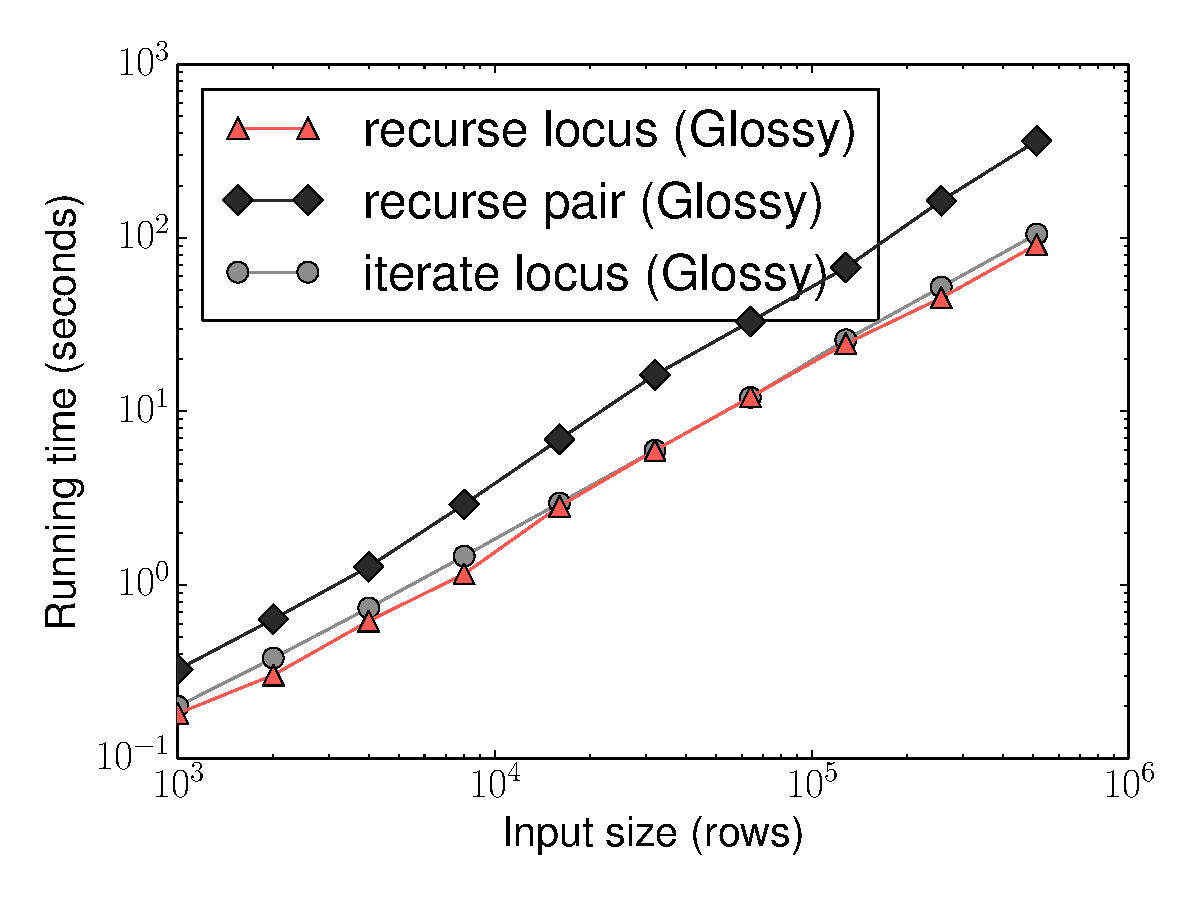
\includegraphics{figs-glossy/scalability.pdf}}
\vspace{-4ex}
\caption{Scalability of three Glossy query-types on POI data: (triangles) recursive query with locus constraint, (diamonds) recursive query with pair constraint, (circles) iterative query with locus constraint.}
\vspace{-3ex}
\label{fig:scalability}
\end{figure}


\begin{figure*}[!t]
     \begin{minipage}{0.32\linewidth}
        \centerline{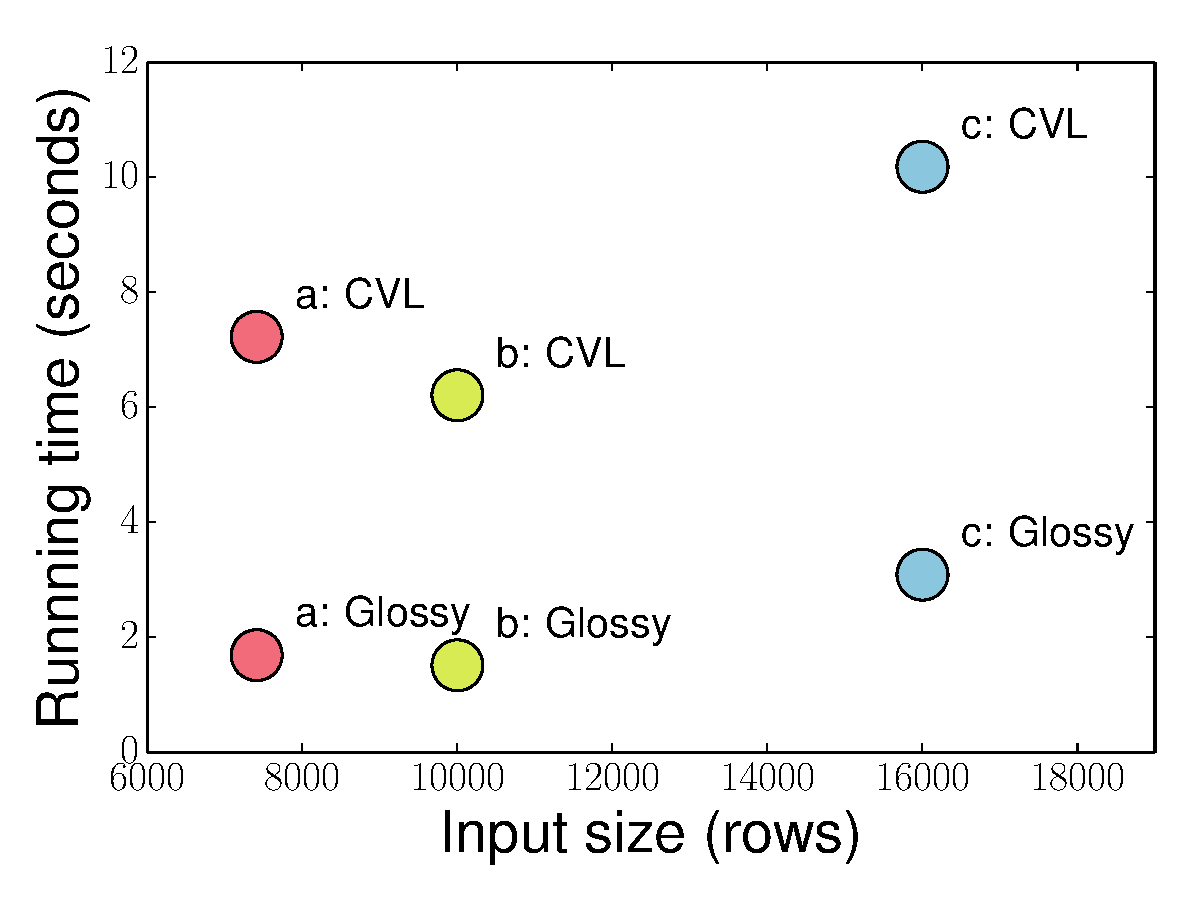
\includegraphics[width=1\linewidth]{figs-glossy/comparison_glossy_vs_cvl_locus.pdf}}
        \vspace{-3ex}
        \caption{Response time of equivalent queries in Glossy vs. CVL with locus constraint: (a) Airports, (b) Placenames, (c) Points of Interest.}\label{fig:glossy:vs:cvl:locus}
    \end{minipage} \hfill
    \begin{minipage}{0.32\linewidth}
        \label{fig:glossy:vs:cvl:pair}
        \centerline{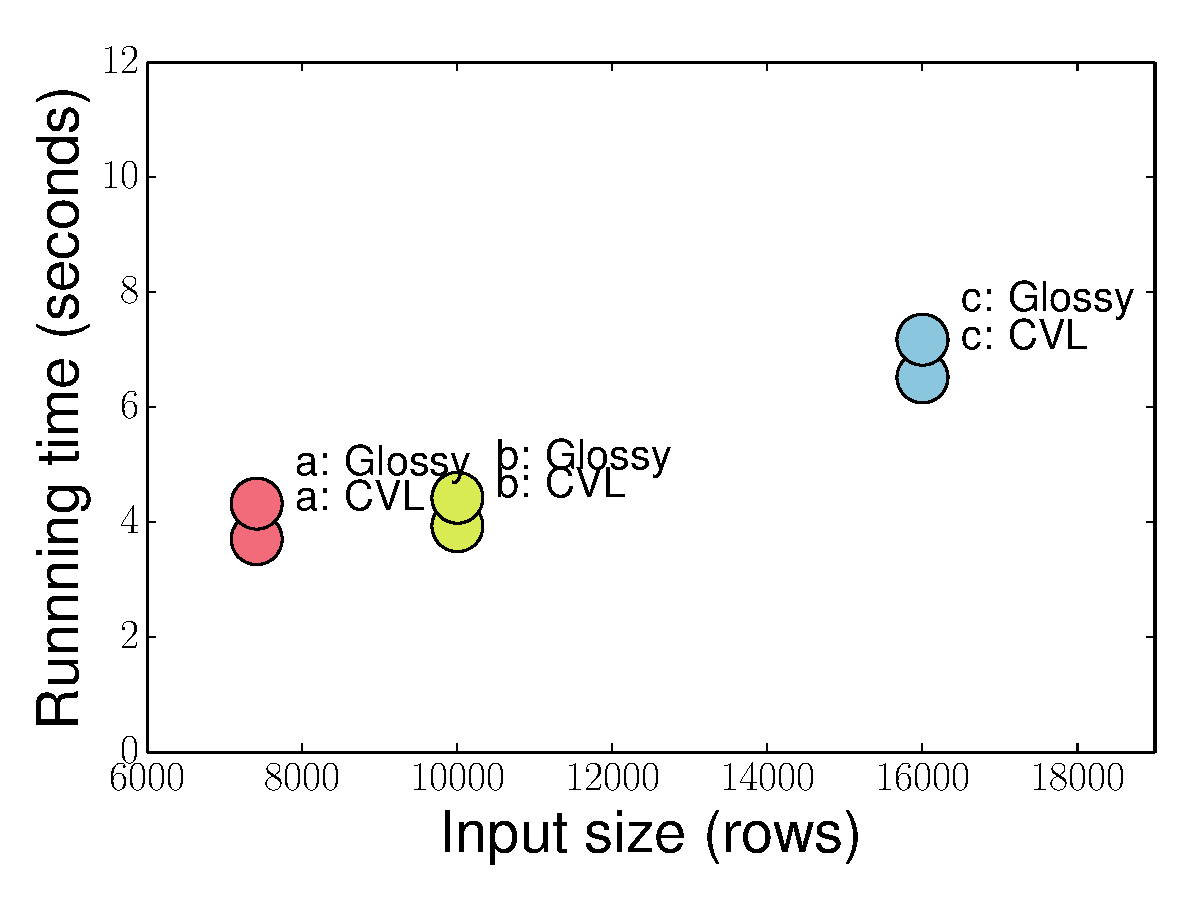
\includegraphics[width=1\linewidth]{figs-glossy/comparison_glossy_vs_cvl_pair.pdf}}
        \vspace{-3ex}
        \caption{Response time of equivalent queries in Glossy vs. CVL with pair constraint: (a) Airports, (b) Placenames, (c) Points of Interest.} \label{fig:glossy:vs:cvl:pair}
    \end{minipage} \hfill
        \begin{minipage}{0.32\linewidth}
        \centerline{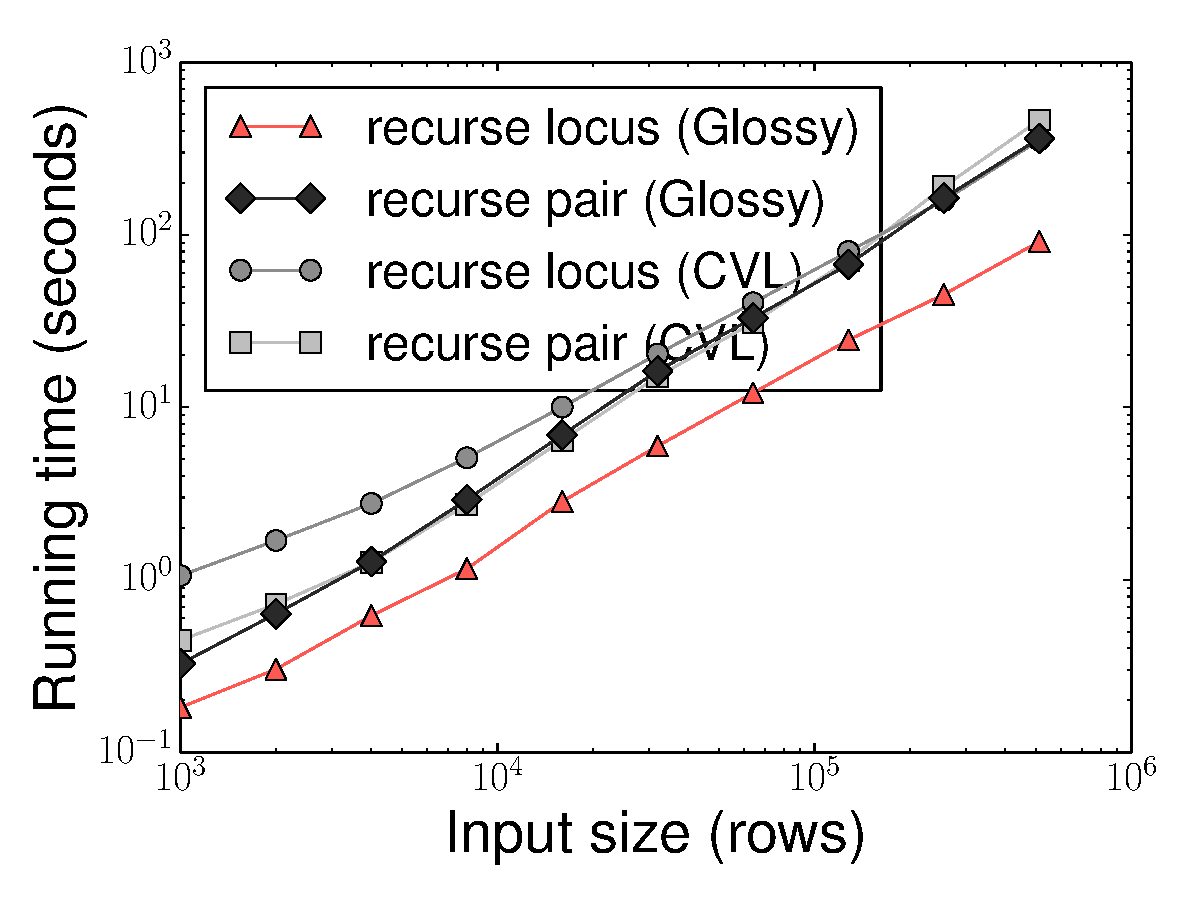
\includegraphics[width=1\linewidth]{figs-glossy/scalability_vs_cvl.pdf}}
        \vspace{-3ex}
        \caption{Scalability of equivalent recursive queries in Glossy vs. CVL with locus and pair constraints on scaled point of interest data.} \label{fig:scalability:glossy:vs:cvl}
    \end{minipage} \hfill
%\vspace{-1ex}
\end{figure*}

\subsection{Scalability}
\label{sec:exp:scalability}

We evaluated the scalability of Glossy SQL by deriving ten POI datasets with between $1000$ and $512000$ records, while attempting to scale dataset size exponentially. We adopt the same scaling procedure described by Kefaloukos et al.~\cite{KefaloukosSZ14:CVL}. A sweep-line approach is employed to enlarge the dataset along the x-axis in the west to east direction. The main property of this procedure is that the size of the dataset can be gradually increased, while maintaining local density. The scalability results are reported in Figure~\ref{fig:scalability}. 

To test a variety of queries, we started from the query of Figure~\ref{fig:glossy:sql:poi} and modified it along two dimensions: (a)~we chose to either use a single locus or pair constraint, and (b)~we chose to either use a \textbf{\texttt{RECURSE OVER}} or an \textbf{\texttt{ITERATE OVER}} clause. The four resulting queries were compiled by Glossy and executed on PostgreSQL. PostgreSQL failed to obtain an efficient query plan for the iterative query with a pair constraint. While the issue could potentially be addressed by manually adding optimizer hints or switching to a more sophisticated query optimizer, we preferred to  run the Glossy and PostgreSQL combination untouched in our experiments and thus omit the results for this particular query. 

Figure~\ref{fig:scalability} shows that the SQL queries generated by the Glossy SQL compiler scale linearly on the input size up to at least 510K data items. The figure also shows a marked difference between queries involving pair and locus constraints. The running times of the recursive query with a pair constraint are consistently worse than of the other two queries throughout the whole range of input sizes evaluated. With a dataset of $512000$ records, the observed response time is higher by a factor of roughly four, reaching close to seven minutes compared to just roughly two minutes for the other query types. The pair constraint involves a notoriously expensive spatial join operation, which we have confirmed to be the dominant factor in the observed differences. Note that Glossy SQL queries compute the entire visualization results for all zoom levels, so we argue that a response time of a few minutes is acceptable for the offline pre-computation of a whole visualization.     


\subsection{Running the Use Cases}

Having established the baseline scalability of SQL queries generated by Glossy, we turn our attention to the use cases discussed in Section~\ref{sec:use:cases} for which Glossy SQL queries have been presented in Section~\ref{sec:use:cases:solved}, Figures~\ref{fig:glossy:sql:rappers}-\ref{fig:glossy:sql:placenames}. We evaluate SQL queries generated by the Glossy SQL compiler over the real datasets of rap lyrics, points of interest, placenames, and the larger, synthetic placenames dataset. 

\begin{table}[ht]
%\vspace{-1ex}
\begin{center}
\tabcolsep=0.11cm
\begin{tabular}{|l|l|l|l|}
\hline
\multirow{2}{*}{\textbf{Use Case}} & \multirow{2}{*}{\textbf{Query}} & \multirow{2}{*}{\textbf{Dataset}} & \textbf{Response} \\
                                                             &                                                      &                                                          & \textbf{Time} \\ 
\hline
UC~\ref{ex:rappers}: Vocabulary Size & Figure~\ref{fig:glossy:sql:rappers} & Rap Lyrics & 157~msec  \\
UC~\ref{ex:poi}: Points of Interest & Figure~\ref{fig:glossy:sql:poi} & Points of Interest & 6.5~min  \\
UC~\ref{ex:placenames}: Placenames & Figure~\ref{fig:glossy:sql:placenames}\footnotemark & Placenames & 1.5~sec \\
UC~\ref{ex:placenames}: Placenames & Figure~\ref{fig:glossy:sql:placenames} & Synthetic Places & 6.6~min  \\
\hline
\end{tabular}
\vspace{-2ex}
\caption{Performance of running use cases with Glossy}
\label{tab:use:cases:performance}
\end{center}
\vspace{-3ex}
\end{table}%

The response times observed for running the use cases are summarized in Table~\ref{tab:use:cases:performance}. We observe that times are strongly correlated with input size and with the types and definitions of constraints employed by the queries. Use Case~\ref{ex:rappers} exhibits the lowest response time, of under a couple hundred milliseconds. This use case employs a Glossy SQL query with only a locus constraint, and is run over a relatively small dataset with $13000$ records. While Use Case~\ref{ex:placenames} is run over a comparatively small dataset, its query employs a locus constraint with more expensive geometric operations to obtain loci than the simple division of Use Case~\ref{ex:rappers}. This difference leads to an execution time roughly one order of magnitude larger. 

\footnotetext{Since the Placenames dataset from GeoNames only includes points, and not polygons for named places, we have changed the query in Figure~\ref{fig:glossy:sql:placenames} by omitting the \textbf{\texttt{WHERE}} clause, and by mapping each point to exactly one tile.}

In spite of the latter, execution times are still low in absolute terms for both small datasets. For the two larger datasets, we observe response times in the order of six to seven minutes. The behavior of Use Case~\ref{ex:poi} is in line with what we have observed in the scalability experiments of Section~\ref{sec:exp:scalability}, since the query employs a pair constraint with a spatial join. For Use Case~\ref{ex:placenames}, we again have the use of complex geometric operations, this time to determine tile centers for named place polygons over a challenging synthetic dataset. We speculate that the use of advanced methods for spatial operations in the underlying database, such as use of parallelism and advanced indexing structures, could speed these queries up by a substantial amount. 

\subsection{Comparison with CVL}

Over the previous sections, we have explored a range of queries and use cases for Glossy SQL. In this section, we focus on comparing Glossy SQL with CVL. Unlike Glossy SQL, CVL neither supports iterative queries nor the specification of an ordered table with information on scales. As such, we focus on recursive queries with range clauses over a fixed number of zoom levels. In addition, CVL requires specification of geometry columns, so we restrict our attention only to use cases in the domain of geographical maps. 

We compare the two systems with the POI and Placenames datasets evaluated previously, as well as the Airports dataset, which was used in the experimental evaluation of Kefaloukos et at.~\cite{KefaloukosSZ14:CVL}. We experiment with two types of recursive queries, namely containing either a single locus or pair constraint. All queries range over an interval of zoom levels $[0,18]$, similarly to Figure~\ref{fig:glossy:sql:poi}. 

Figures~\ref{fig:glossy:vs:cvl:locus} and~\ref{fig:glossy:vs:cvl:pair} show the results for both systems. We observe that for queries involving only a locus constraint, the performance of Glossy is substantially superior to that of CVL, exhibiting running times lower by over a factor of three. This result suggests that the SQL translation employed by Glossy for these queries is not only more general, but also more performant than the translation employed by CVL. For queries involving a pair constraint, however, the running time of both systems is comparable. This behavior is in line with our observation that the spatial join in the pair constraint essentially dominates the running time.        

To complete our evaluation, we have run a scalability experiment with the two systems, with a setup similar to the one of Section~\ref{sec:exp:scalability}. However, we focused only on the query types explored in this section, given the restrictions of CVL. The results are shown in Figure~\ref{fig:scalability:glossy:vs:cvl}. We can see that both systems scale linearly with the input size. That being said, we observe again in this experiment the performance trends above: For a locus constraint, the performance of Glossy is superior across the whole range of input sizes, while for a pair constraint involving a spatial join the performance of the two systems is comparable. 

From this evaluation, we observe that Glossy generally dominates CVL, not only in terms of expressivity, but also performance.  

% what to compare against?
% Selling points:
% - Global Selection: leaving minute data selection to system 
% Goal of experiment: Show that Global Selection can be implemented efficiently

\section{Conclusions}

In this paper, we argue for and propose an extension of SQL to express global selection operations, motivated by a wealth of use cases in data visualization. Global selections sample records from a dataset in a way that is at the same time constrained and weighted. The paper presents a concrete system, Glossy, that processes global selection queries by translating them to pure SQL and running the resulting queries over existing RDBMS. Glossy SQL allows for the declarative expression of both pair and locus constraints over the dataset, of a weighting function for records, and of both iterative and recursive global selections. The latter features let visualization developers express record importance as well as visual conflicts to be avoided in a manner sensitive to scale in a zoomable visualization. Experimental results with the Glossy SQL translation of several visualization use cases indicate that Glossy generates SQL code that an existing RDBMS can execute both efficiently and scalably with increasing input sizes. 

As future work, we plan to explore how to incorporate data aggregation features into Glossy SQL, as well as integrate Glossy with an existing library of visualization components such as D3.\footnote{http://d3js.org/}
